% This is "sig-alternate.tex" V2.0 May 2012
% This file should be compiled with V2.5 of "sig-alternate.cls" May 2012
%
% This example file demonstrates the use of the 'sig-alternate.cls'
% V2.5 LaTeX2e document class file. It is for those submitting
% articles to ACM Conference Proceedings WHO DO NOT WISH TO
% STRICTLY ADHERE TO THE SIGS (PUBS-BOARD-ENDORSED) STYLE.
% The 'sig-alternate.cls' file will produce a similar-looking,
% albeit, 'tighter' paper resulting in, invariably, fewer pages.
%
% ----------------------------------------------------------------------------------------------------------------
% This .tex file (and associated .cls V2.5) produces:
%       1) The Permission Statement
%       2) The Conference (location) Info information
%       3) The Copyright Line with ACM data
%       4) NO page numbers
%
% as against the acm_proc_article-sp.cls file which
% DOES NOT produce 1) thru' 3) above.
%
% Using 'sig-alternate.cls' you have control, however, from within
% the source .tex file, over both the CopyrightYear
% (defaulted to 200X) and the ACM Copyright Data
% (defaulted to X-XXXXX-XX-X/XX/XX).
% e.g.
% \CopyrightYear{2007} will cause 2007 to appear in the copyright line.
% \crdata{0-12345-67-8/90/12} will cause 0-12345-67-8/90/12 to appear in the copyright line.
%
% ---------------------------------------------------------------------------------------------------------------
% This .tex source is an example which *does* use
% the .bib file (from which the .bbl file % is produced).
% REMEMBER HOWEVER: After having produced the .bbl file,
% and prior to final submission, you *NEED* to 'insert'
% your .bbl file into your source .tex file so as to provide
% ONE 'self-contained' source file.
%
% ================= IF YOU HAVE QUESTIONS =======================
% Questions regarding the SIGS styles, SIGS policies and
% procedures, Conferences etc. should be sent to
% Adrienne Griscti (griscti@acm.org)
%
% Technical questions _only_ to
% Gerald Murray (murray@hq.acm.org)
% ===============================================================
%
% For tracking purposes - this is V2.0 - May 2012



\documentclass{acm_proc_article-me}

\usepackage[utf8]{inputenc}
\usepackage[T1]{fontenc}

\usepackage{amssymb}
\usepackage{amsfonts}
\usepackage{url}

\newcommand\queries{\mathbb{Q}}

\newcommand\refEvidences{\mathbb{E}}
\newcommand\refLabels{\mathbb{L}}
\newcommand\refNames{\mathbb{N}}
\newcommand\shots{\mathbb{S}}

\newcommand\hypEvidences{\mathcal{E}}
\newcommand\hypLabels{\mathcal{L}}
\newcommand\hypNames{\mathcal{N}}

\newcommand\ratio{\rho}

\DeclareMathOperator*{\argmax}{arg\,max}
\DeclareMathOperator*{\argmin}{arg\,min}

\begin{document}
%
% --- Author Metadata here ---

%Copyright is held by the author/owner(s).

\conferenceinfo{\textit{MediaEval 2016 Workshop,}}{Oct. 20-21, 2016, Hilversum, Netherlands.}

%\conferenceinfo{WOODSTOCK}{'97 El Paso, Texas USA}
%\CopyrightYear{2007} % Allows default copyright year (20XX) to be over-ridden - IF NEED BE.
%\crdata{0-12345-67-8/90/01}  % Allows default copyright data (0-89791-88-6/97/05) to be over-ridden - IF NEED BE.
% --- End of Author Metadata ---

\title{Multimodal Person Discovery in Broadcast TV\\at MediaEval 2016}
%
% You need the command \numberofauthors to handle the 'placement
% and alignment' of the authors beneath the title.
%
% For aesthetic reasons, we recommend 'three authors at a time'
% i.e. three 'name/affiliation blocks' be placed beneath the title.
%
% NOTE: You are NOT restricted in how many 'rows' of
% "name/affiliations" may appear. We just ask that you restrict
% the number of 'columns' to three.
%
% Because of the available 'opening page real-estate'
% we ask you to refrain from putting more than six authors
% (two rows with three columns) beneath the article title.
% More than six makes the first-page appear very cluttered indeed.
%
% Use the \alignauthor commands to handle the names
% and affiliations for an 'aesthetic maximum' of six authors.
% Add names, affiliations, addresses for
% the seventh etc. author(s) as the argument for the
% \additionalauthors command.
% These 'additional authors' will be output/set for you
% without further effort on your part as the last section in
% the body of your article BEFORE References or any Appendices.

\numberofauthors{1}

\author{
% You can go ahead and credit any number of authors here,
% e.g. one 'row of three' or two rows (consisting of one row of three
% and a second row of one, two or three).
%
% The command \alignauthor (no curly braces needed) should
% precede each author name, affiliation/snail-mail address and
% e-mail address. Additionally, tag each line of
% affiliation/address with \affaddr, and tag the
% e-mail address with \email.
%
% 1st. author
\alignauthor
Herv\'e Bredin, Claude Barras, Camille Guinaudeau \\
       \affaddr{LIMSI, CNRS, Univ. Paris-Sud, Universit\'e Paris-Saclay, F-91405 Orsay, France.}
       \email{firstname.lastname@limsi.fr}
\\
}
% There's nothing stopping you putting the seventh, eighth, etc.
% author on the opening page (as the 'third row') but we ask,
% for aesthetic reasons that you place these 'additional authors'
% in the \additional authors block, viz.
\date{13 July 2016}
% Just remember to make sure that the TOTAL number of authors
% is the number that will appear on the first page PLUS the
% number that will appear in the \additionalauthors section.

\maketitle
\begin{abstract}
We describe the ``Multimodal Person Discovery in Broadcast TV'' task of MediaEval 2016 benchmarking initiative. Participants are asked to return the names of people who can be both seen as well as heard in every shot of a collection of videos. The list of people is not known \emph{a priori} and their names has to be discovered in an unsupervised way from media content using text overlay or speech transcripts for the primary runs. The task is evaluated using information retrieval metrics, based on \emph{a posteriori} collaborative annotation of the test corpus.
\end{abstract}

\vspace{-0.1cm}
\section{Motivation}

TV archives maintained by national institutions such as the French INA, the Netherlands Institute for Sound \& Vision, or the British Broadcasting Corporation are rapidly growing in size. The need for applications that make these archives searchable has led researchers to devote concerted effort to developing technologies that create indexes.

Indexes that represent the location and identity of people in the archive are indispensable for searching archives. Human nature leads people to be very interested in other people. However, when the content is created or broadcasted, it is not always possible to predict which people will be the most important to find in the future
and biometric models may not yet be available at indexing time
The goal of this task is thus to address the challenge of indexing people in the archive under real-world conditions, \emph{i.e.}, when there is no pre-set list of people to index.

%Early approaches relying on pronounced names instead of biometric models for speaker identification~\cite{CANSECO--ASRU--2005, CANSECO--INTERSPEECH--2004, ESTEVE--INTERSPEECH--2007, JOUSSE--ICCASP--2009, MAUCLAIR--Odyssey--2006, TRANTER--ICASSP--2006} were hampered by relatively high speech transcription errors or and named entity detection errors. Similarly, initial visual-only approaches based on overlaid title box transcriptions for face recognition were very dependent on the quality of overlaid name transcription~\cite{HOUGHTON--IS--1999, SATOH--IEEEMM--1999, YANG--ACMMM--2004, YANG--ACMMM--2005}.
Started in 2011, the REPERE challenge aimed at supporting research on multimodal person recognition~\cite{BERNARD--SLAM--2013, KAHN--CBMI--2012}. Its main goal was to answer the two questions \emph{``who speaks when?''} and \emph{``who appears when?''} using any available source of information (including pre-existing biometric models and person names extracted from text overlay and speech transcripts). Thanks to this challenge and the associated multimodal corpus~\cite{GIRAUDEL--LREC--2012}, significant progress was achieved in either supervised or unsupervised multimodal person recognition~\cite{BECHET--INTERSPEECH--2014, BENDRIS--CBMI--2013, BREDIN--ODYSSEY--2014, BREDIN--INTERSPEECH--2013, BREDIN--SLAM--2013, BREDIN--IJMIR--2014, FAVRE--SLAM--2013, GAY--CBMI--2014, POIGNANT--ASLP--2015, POIGNANT--SLAM--2013, POIGNANT--INTERSPEECH--2012, POIGNANT--MTAP--2015, ROUVIER--CBMI--2014}.
After the end of the REPERE challenge in 2014, the  first edition of the ``Multimodal Person Discovery in Broadcast TV'' task was organized in 2015 \cite{POIGNANT--MEDIAEVAL--2015}. This year's task is a follow-up of last year edition.

\vspace{-0.1cm}
\section{Definition of the task}

Participants are provided with a collection of TV broadcast recordings pre-segmented into shots.
Each shot $s \in \shots$ has to be automatically tagged with the names of people both speaking and appearing at the same time during the shot: this tagging algorithm is denoted by $\hypLabels : \shots \mapsto \mathcal{P}(\hypNames)$ in the rest of the paper.
As last year, the list of persons is not provided \emph{a priori}, and person biometric models (neither voice nor face) can not be trained on external data in the primary runs. The only way to identify a person is by finding their name $n \in \hypNames$ in the audio (\emph{e.g.} using speech transcription -- ASR) or visual (\emph{e.g.} using optical character recognition -- OCR) streams and associating them to the correct person. This makes the task completely unsupervised (\emph{i.e.} using algorithms not relying on pre-existing labels or biometric models). The main novelty of this year task is that participants may use their contrastive run to try brave new ideas that may rely on any external data, including textual metadata provided with the test set.

Because person names are detected and transcribed automatically, they may contain transcription errors to a certain extent (more on that later in Section~\ref{sec:metric}). In the following, we denote by $\refNames$ the set of all possible person names in the universe, correctly formatted as \texttt{firstname\_lastname} -- while $\hypNames$ is the set of hypothesized names.

\begin{figure}[!htb]
 \centering
 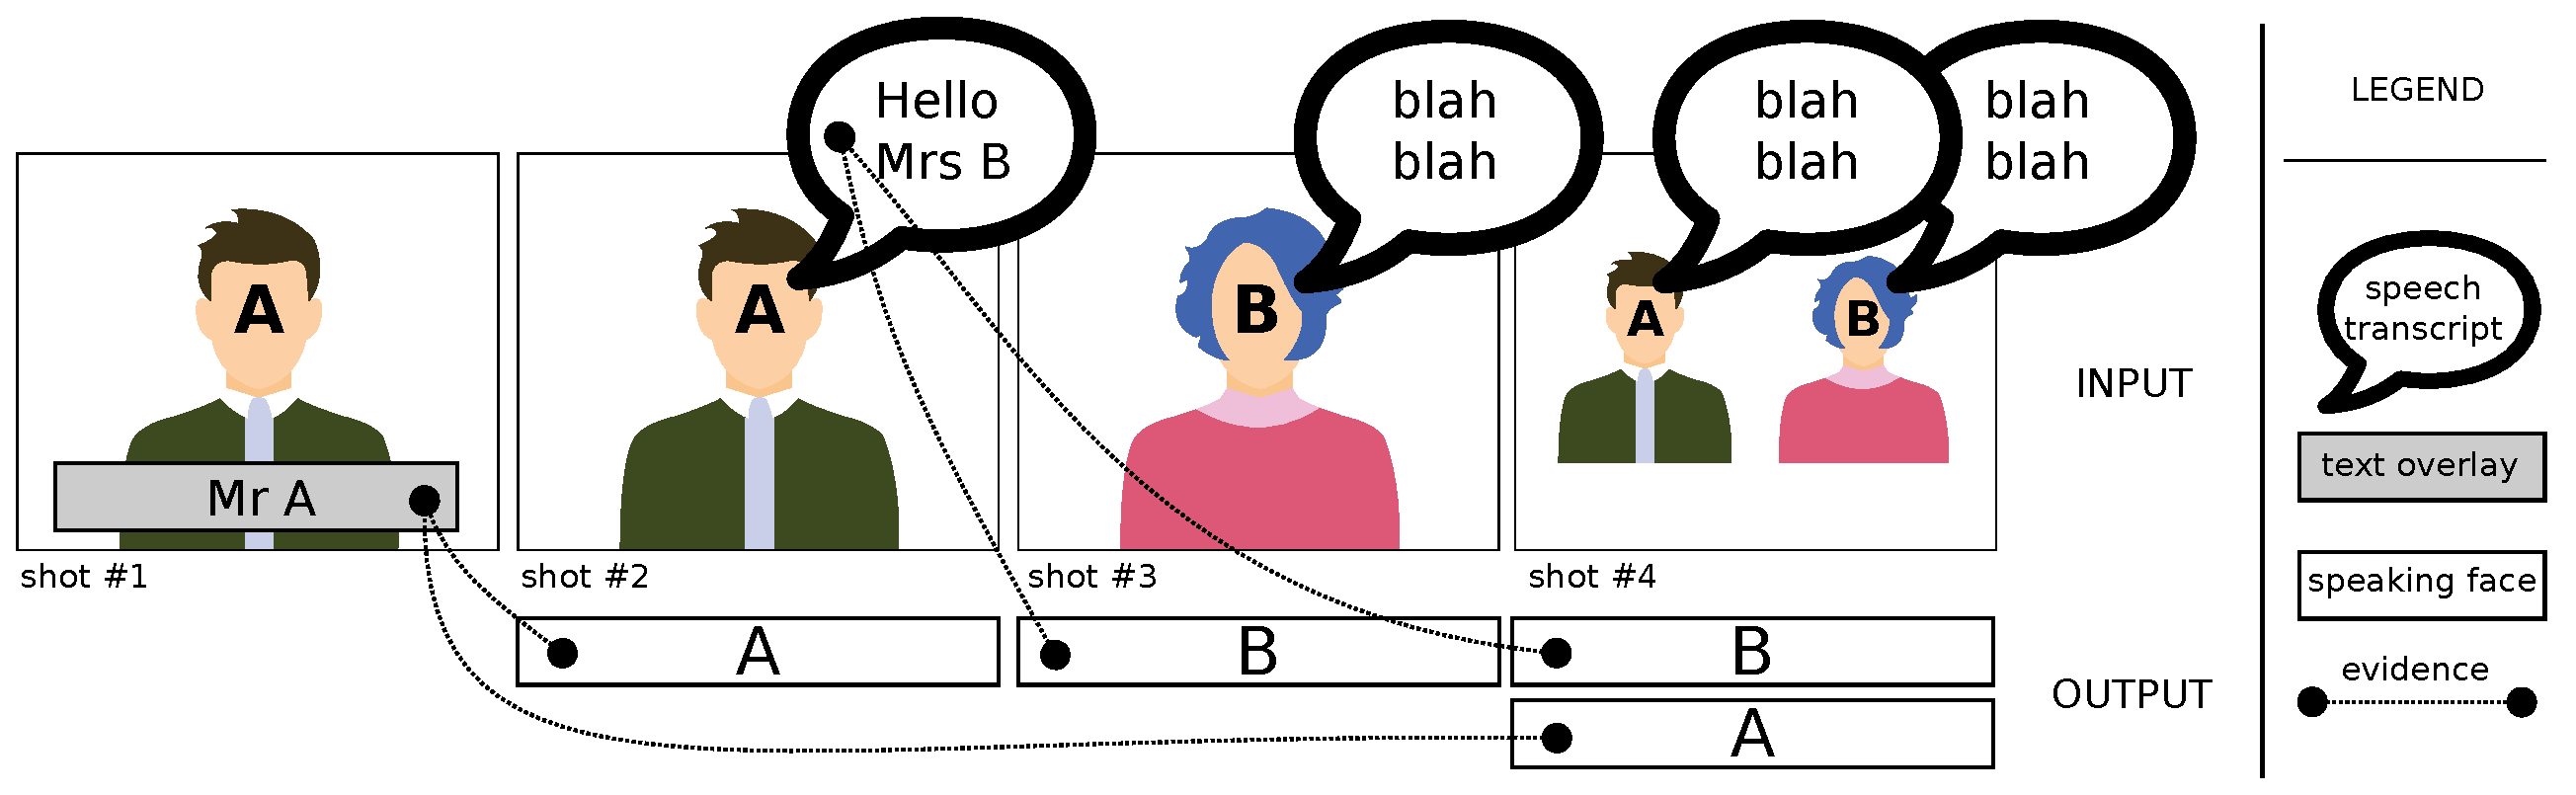
\includegraphics[width=1.\linewidth]{figs/evidence.pdf}
 \vspace{-0.5cm}
 \caption{For each shot, participants have to return the names of every speaking face. Each name has to be backed up by an evidence.}
 \label{fig:evidence}
\end{figure}

\vspace{-0.1cm}
\section{Datasets}

The 2015 test corpus serves as development set for this year's task. It contains 106 hours of video, corresponding to 172 editions of evening broadcast news \emph{``Le 20 heures''} of French public channel \emph{``France 2''}, from January 1st 2007 to June 30st 2007. This development set is associated with \emph{a posteriori} annotations based on last year participants' submissions. 

The test set is divided into three datasets: INA, DW and 3-24. The INA dataset contains a full week of broadcast for 3 TV channels and 3 radio channels in French. Only a subset (made of 2 TV video channels for a total duration of 90 hours) needs to be processed. However, participants can process the rest of it if they think it might lead to improved results. Moreover, this dataset is associated with manual metadata provided by INA in the shape of CSV files. The DW dataset is composed of video downloaded from Deutsche Welle website, in English and German for a total duration of 50 hours. This dataset is also associated with medata that can be used in contrastive runs. The last dataset contains 13 hours of broadcast from 3/24 Catalan TV news channel.

As the test set comes completely free of any annotation, it will be annotated \emph{a posteriori} based on participants' submissions. 
In order to ease this annotation process, participants are asked to justify their assertion. To this end, each hypothesized name $n \in \hypNames$ has to be backed up by a carefully selected and unique shot prooving that the person actually holds this name $n$: we call this an evidence and denote it by $\hypEvidences : \hypNames \mapsto \shots$. In real-world conditions, this evidence would help a human annotator double-check the automatically-generated index, even for people they did not know beforehand.

Two types of evidence are allowed: an \emph{image} evidence is a time in a video when a person is visible, while his/her name is written on screen; an \emph{audio} evidence is the time when the name of a person is pronounced, provided that this person is visible in a $[\text{time} - 5s, \text{time} + 5s ]$ neighborhood.
For instance, in Figure~\ref{fig:evidence}, shot \#1 contains an \emph{image} evidence for Mr A (because his name and his face are visible simultaneously on screen) while shot \#3 contains an \emph{audio} evidence for Mrs B (because her name is pronounced less than 5 seconds before or after her face is visible on screen).

In the following, task groundtruths are denoted by function $\refLabels : \shots \mapsto \mathcal{P}(\refNames)$ that maps each shot $s$ to the set of names of every speaking face it contains, and function $\refEvidences : \shots \mapsto \mathcal{P}(\refNames)$ that maps each shot $s$ to the set of person names for which it actually is an evidence.

\vspace{-0.1cm}
\section{Baseline and metadata}

This task target researchers from several communities including multimedia, computer vision, speech and natural language processing. Though the task is multimodal by design and necessitated expertise in various domains, the technological barriers to entry is lowered by the provision of a baseline system described in Figure~\ref{fig:baseline} and available as open-source software\footnote{\url{http://github.com/MediaEvalPersonDiscoveryTask}}.
For instance, a researcher from the speech processing community can focus its research efforts on improving speaker diarization and automatic speech transcription, while still being able to rely on provided face detection and tracking results to participate to the task.

\begin{figure}[htb]
 \centering
 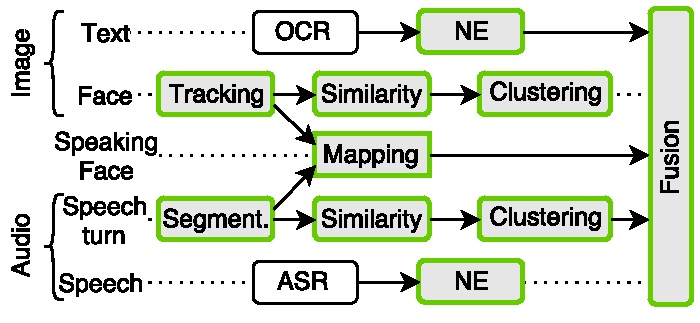
\includegraphics[width=0.95\linewidth]{figs/baseline.pdf}
 \vspace{-0.6cm}
 \caption{Multimodal baseline pipeline. Output of greyed out modules is provided to the participants.}
 \label{fig:baseline}
\end{figure}

The audio stream is segmented into speech turns, while faces are detected and tracked in the visual stream.
Speech turns (resp. face tracks) are then compared and clustered based on MFCC and the Bayesian Information Criterion~\cite{CHEN--DARPA--1998} (resp. HOG~\cite{DALAL--CVPR--2005} and Logistic Discriminant Metric Learning~\cite{GUILLAUMIN--JCV--2012} on facial landmarks~\cite{URICAR--VISAPP--2012}). The approach proposed in~\cite{POIGNANT--MTAP--2015} is also used to compute a probabilistic mapping between co-occuring faces and speech turns. Written (resp. pronounced) person names are automatically extracted from the visual stream (resp. the audio stream) using Optical Character Recognition (resp. Automatic Speech Recognition) followed by Named Entity detection (NE). Speaker diarization and speech transcription for French, German and English are contributed by LIUM~\cite{ROUVIER--INTERSPEECH--2013, GUPTA--ASRU--2015} while OCR is contributed by IDIAP and UPC. The fusion module is a two-steps algorithm: propagation of written names onto speaker clusters~\cite{POIGNANT--INTERSPEECH--2012} followed by propagation of speaker names onto co-occurring speaking faces.

\vspace{-0.1cm}
\section{Evaluation metric}
\label{sec:metric}

This information retrieval task is evaluated using Mean Average Precision (MAP).
For each query $q \in \queries \subset \refNames$ (\texttt{first\-name\_lastname}), the hypothesized person name $n_q$ with the highest Levenshtein ratio $\rho$ to the query $q$ is selected ($\ratio : \refNames \times \hypNames \mapsto [0, 1]$) -- allowing approximate name transcription:
\begin{align}
\displaystyle n_q & = \argmax_{n \in \hypNames} \rho\left(q, n \right) \text{ and } \rho_q = \rho\left(q, n_q \right) \nonumber \\
\intertext{Average precision $\text{AP}(q)$ is then computed classically based on relevant and returned shots:}
\text{relevant}(q) & = \{ s \in \shots \;|\; q \in \refLabels(s) \} \nonumber \\
\text{returned}(q) & = {\{ s \in \shots \;|\; n_q \in \hypLabels(s) \}}_{\begin{subarray}{l}\text{sorted by}\\
    \text{confidence}\end{subarray}} \nonumber \\
\intertext{Mean Average Precision is then computed as follows:}
            \text{MAP} & = \frac{1}{|\queries|} \sum_{q \in \queries} \text{AP}(q) \nonumber
\end{align}

\noindent\textbf{Acknowledgment.} This work was supported by the French National Agency for Research under grants ANR-12-CHRI-0006-01 and ANR-14-CE24-0024. The open source CAMO\-MILE collaborative annotation platform\footnote{\url{http://github.com/camomile-project}} was used extensively throughout the progress of the task: from the run submission script to the automated leaderboard, including \emph{a posteriori} collaborative annotation of the test corpus.
The task builds on Johann Poignant involvement in 2015 task organization.
Xavier Trimolet helped design and develop the 2016 annotation interface.
We also thank INA for supporting the task by distributing development and test datasets, Sylvain Meignier and Yannick Est\`eve from LIUM for providing the ASR and diarization of most corpora, Ramon Morros and Javier Hernando from UPC for contributing the 3/24 TV corpus along with its transcription and OCR, Nam Le and Jean-Marc Odobez from IDIAP for contributing the DW corpus gathered during the EUMSSI project and for the OCR.

\newpage


% The following two commands are all you need in the
% initial runs of your .tex file to
% produce the bibliography for the citations in your paper.
\bibliographystyle{abbrv}
\bibliography{publi}  % sigproc.bib is the name of the Bibliography in this case
% You must have a proper ".bib" file
%  and remember to run:
% latex bibtex latex latex
% to resolve all references


\end{document}
